% statistics_and_probability:x09 GDC:NO
\begin{question}
  \hspace*{\fill} [Note maximale: TBD]\par
  \medskip
  \noindent Les couleurs des yeux de 97 élèves sont données dans le tableau suivant.\par
  \medskip  
  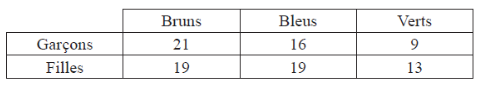
\includegraphics[scale=0.7]{tableau_yeux}\par  
  \medskip
  \noindent Un elève est choisi au hasard.\par
  (a) Donnez la probabilité que cet élève soit un garçon.\hspace*{\fill} [TBD]\par

  (b) Donnez la probabilité que cet élève ait les yeux verts, sachant qu’il s’agit d’une fille.\hspace*{\fill} [TBD]\par

  (c) Trouvez la probabilité que cet élève ait les yeux verts ou soit un garçon.\hspace*{\fill} [TBD]\par
  

\end{question}

